\documentclass[conference]{IEEEtran}
\IEEEoverridecommandlockouts
% The preceding line is only needed to identify funding in the first footnote. If that is unneeded, please comment it out.
\usepackage{cite}
\usepackage{amsmath,amssymb,amsfonts}
\usepackage{algorithmic}
\usepackage{graphicx}
\usepackage{textcomp}
\usepackage{hyperref}
\usepackage{xcolor}

\def\BibTeX{{\rm B\kern-.05em{\sc i\kern-.025em b}\kern-.08em
    T\kern-.1667em\lower.7ex\hbox{E}\kern-.125emX}}
\begin{document}

\title{Simple Reactive Robot\\
}

\author{

    \IEEEauthorblockN{Carlos Veríssimo}
    \IEEEauthorblockA{\textit{Department of Informatics Engineering} \\
        \textit{FEUP}\\
        Porto, Portugal \\
        up201907716@up.pt }
    \and

    \IEEEauthorblockN{Miguel Amorim}
    \IEEEauthorblockA{\textit{Department of Informatics Engineering } \\
        \textit{FEUP}\\
        Porto, Portugal \\
        up201907756@up.pt }
    \and

    \IEEEauthorblockN{Rafael Camelo}
    \IEEEauthorblockA{\textit{Department of Informatics Engineering } \\
        \textit{FEUP}\\
        Porto, Portugal \\
        up201907729@up.pt }
}


\maketitle

\begin{abstract}

    In an era defined by dynamic and ever-evolving technological landscapes, the development of a REACTIVE (Real-time, Environment-Adaptive, and Contextually-Intelligent) robot under the aegis of the Robot Operating System (ROS) represents a pivotal step forward in the realm of robotics. This ambitious project aspires to create a robotic entity with unparalleled adaptability, reactivity, and intelligence in response to its environment.  The simulation is performed in ROS, which runs the Python code and integrates it with the Gazebo simulation
    environment. The reactive robot is generated in a random start
    position. It can successfully follow the wall, avoid hitting, and stop
    in the desired end position.

\end{abstract}

\begin{IEEEkeywords}
    Robotics, Intelligent, ROS, Gazebo, Simulation, Sensor, Actuator, Navigation, Environment
\end{IEEEkeywords}

\section{Introduction}
As technology continues to advance, autonomous mobile robots are increasingly finding applications across various sectors, including corporate environments, industrial settings, healthcare facilities, educational institutions, agriculture, and even in everyday households.
In the context of mobile robot navigation, many scenarios require the implementation of wall-following behaviors. These behaviors allow the robot to navigate along the contours of walls or obstacles while maintaining a safe and consistent distance from them. These autonomous robots exhibit the capability to operate in diverse environments, which can be characterized by non-linearity and partially real-time observations. To address challenges of this nature, a multitude of techniques and solutions have been explored and studied.



\section{State of the Art}

Robot navigation is a fundamental aspect of robotics that focuses on enabling robots to move autonomously and safely in their environment. It involves the development of algorithms, sensors, and control systems to guide robots in tasks such as exploration, mapping, path planning, and obstacle avoidance. Here are some key aspects of robot navigation: \textbf{Sensors -} Robots rely on a variety of sensors to perceive their surroundings. These sensors include cameras, LIDAR (Light Detection and Ranging), ultrasonic sensors, inertial measurement units (IMUs), encoders, and more. These sensors provide data on the robot's position, orientation, and the presence of obstacles. \textbf{Simultaneous Localization and Mapping (SLAM)}: SLAM is a critical technology in robot navigation. It enables a robot to build a map of its environment while simultaneously determining its own position within that environment. This is essential for autonomous navigation and exploration.\textbf{ Path Planning}: Path planning algorithms help robots find a safe and efficient route from their current location to a target destination while avoiding obstacles. These algorithms take into account the environment's layout and the robot's physical constraints. \textbf{Local vs. Global Navigation}: Robots often employ a combination of local and global navigation strategies. Local navigation focuses on short-term decisions, like avoiding immediate obstacles, while global navigation involves planning routes to long-term goals. \textbf{Reactive vs. Deliberative Navigation}: Reactive navigation involves immediate reactions to sensory input, while deliberative navigation considers a broader context and plans actions in advance. Many robots use a combination of both. \textbf{Dynamic Environments}: Navigating in dynamic environments with moving objects or people requires advanced navigation systems that can predict and adapt to changes in real time. \par
Robot navigation is a complex and evolving field with applications in areas such as autonomous vehicles, industrial automation, search and rescue, space exploration, and agriculture. As technology continues to advance, robots are becoming increasingly capable of navigating a wide range of environments and scenarios.


\section{Robot Implementation and Architecture}

\subsection{Robot Specification}

For the implementation of the reactive robot, a simulated version of the Turtlebot3 \footnote{\url{https://www.turtlebot.com/turtlebot3/}}
robot. Throughout the development, we mostly used the \emph{burger} model of Turtlebot3 to test our simulation, however, one can change the model
just by using a different environment variable. More on that in section \ref{sec:run}.

The robot is equipped with a LIDAR sensor, which is used to detect the distance to the walls and obstacles.
The robot also has two wheels, controlled by the \emph{wheel\_left\_joint} and \emph{wheel\_right\_joint} joints.

Figure \ref{fig:robot-comparision} shows the Turtlebot3 Burger in the real world and its simulated counterpart
in Gazebo.

\begin{figure}[h]
    \centering
    \begin{minipage}{.4\columnwidth}
        \centering
        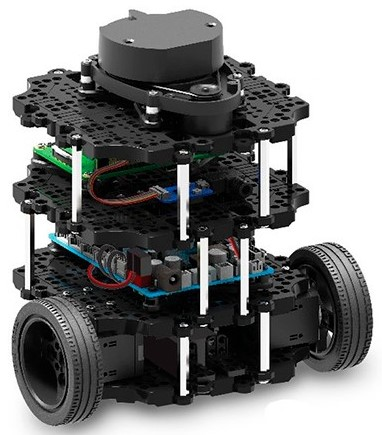
\includegraphics[width=\textwidth]{images/turtlebot3-burger.jpg}
    \end{minipage}%
    \begin{minipage}{.4\columnwidth}
        \centering
        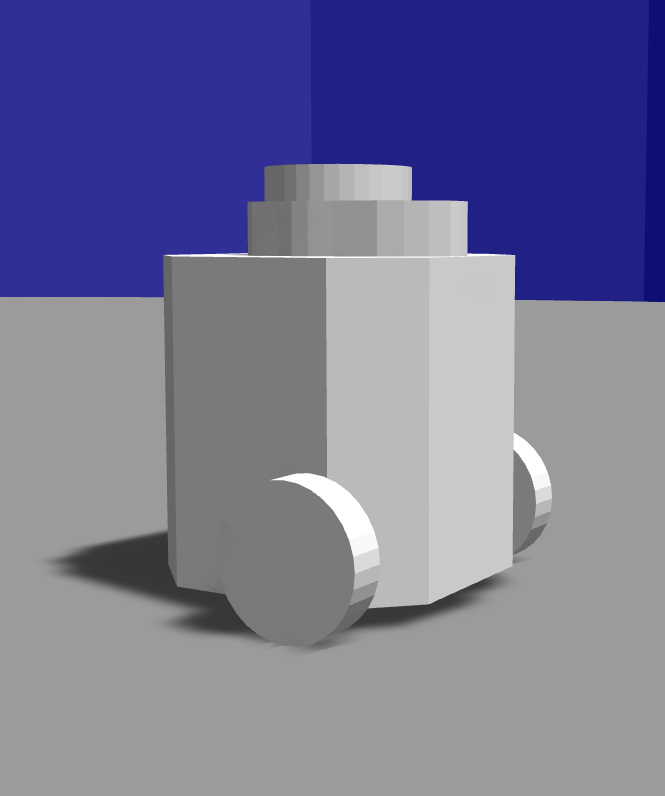
\includegraphics[width=\textwidth]{images/turtlebot3-burger-gazebo.png}
    \end{minipage}
    \label{fig:robot-comparision}
    \caption{Turtlebot3 Burger in the real world (left) and in Gazebo (right)}
\end{figure}

\subsection{The Environment}

The simulation environment is a question-marked shaped world. It was created using the Gazebo building
editor tool.

Project specifications specify that the bottom is straight with an edgy shape.

Below is a visualization of the environment, in Gazebo:

\begin{figure}[h]
    \centering
    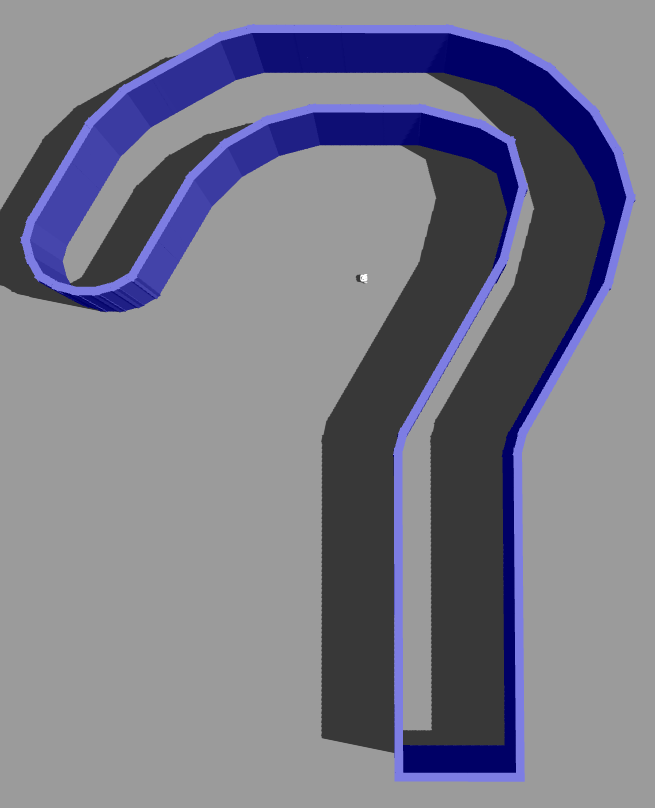
\includegraphics[width=0.3\textwidth]{images/world.png}
    \caption{The simulation world}
    \label{fig:environment}
\end{figure}

\subsection{Packages}

Inside our workspace, two packages were created: \emph{my\textunderscore reactive\textunderscore robot} and \emph{my\textunderscore controller}.

The first package:
\begin{itemize}
    \item Launches Gazebo, by running both \emph{gzserver.launch.py} and \emph{gzclient.launch.py}
    \item Publishes the robot state with the \emph{robot\textunderscore state\textunderscore publisher} node
    \item Spawns our Turtlebot3 robot in the simulation environment, with the \emph{spawn\textunderscore entity.py} service,
          from the package \emph{gazebo\textunderscore ros}
\end{itemize}

The second package, as the name suggests, is responsible for controlling the robot. It contains the following nodes:
\begin{itemize}
    \item \emph{scan\textunderscore to\textunderscore velocity\textunderscore node}: This node subscribes to
          the \emph{scan} topic, which contains the LIDAR data, and publishes the velocity commands to
          the \emph{cmd\textunderscore vel} topic, which controls the robot's wheels.
    \item \emph{spin \textunderscore randomly \textunderscore node}: This node is a workaround that we created to allow for a random initial
          robot orientation. It spins the robot randomly for a few seconds and then stops it.
\end{itemize}

The robot's initial position and pose are random, but are constrained to the round area of the question mark.

\subsection{How to Run the Simulation}\label{sec:run}

To run the simulation, you will need the following ROS packages/dependencies:

\begin{itemize}
    \item \emph{turtlebot3\textunderscore gazebo}: This package contains the Turtlebot3 models and the Gazebo plugins.
    \item \emph{gazebo\textunderscore ros}: This package contains the Gazebo ROS interface.
\end{itemize}

Assure that you have the necessary dependencies and that you have sourced your ROS distribution's setup file. Please refer to the README file in the \href{https://github.com/carlosverissimo3001/FEUP-RI-PROJ/}{project's repository}, if you're having any issues with this process.

\vskip 0.1in

\textbf{Build the package and source the setup file}:

\begin{enumerate}
    \item \texttt{cd FEUP-RI-PROJ} - Go to the project's root directory
    \item \texttt{colcon build --symlink-install} - Build the packages
    \item \texttt{source install/setup.bash} - Source the setup file
    \item \texttt{export TURTLEBOT3\textunderscore MODEL=burger} - Set the Turtlebot3 model.
          You can change this to \emph{waffle} or \emph{waffle\textunderscore pi.}
\end{enumerate}

\vskip 0.1in

\textbf{Run the simulation}:


\begin{enumerate}
    \item Open two terminal windows.
    \item Run \texttt{ros2 launch my\textunderscore reactive\textunderscore robot launch.py} in one of them.
\end{enumerate}

This will launch Gazebo and spawn the robot in the simulation environment. Please wait for Gazebo to load before running
the next command.

In the other terminal window, run \texttt{ros2 run my\textunderscore controller controller\textunderscore node}.
This will launch the nodes that control the robot.

\vskip 0.1in

Please note that we set up Gazebo so that it starts with a paused state. This means that the simulation will not start
until you press the play button in Gazebo's GUI.

\subsection{Implementation}

%% EXPLICAR O CÓDIGO BASICAMENTE

\section{Experiments}

%% Explicar que temos o robot a spwanar em posições aleatórias e com orientações aleatórias.
%% Podemos tambem falar do que acontece quando ele tá perdido (not sure about this one)

\section{Results and Discussion}

%% Loop time, travelled path, performance,
%% discuss stuck robot, control, performance improvement...


\section{Conclusions and Future Work}

%% MENCIOANR PROBLEMAS A CORRER O ROS E GAZEBO

\section{Acknowledgments}

%% NO FUCKING CLUE HERE

\begin{thebibliography}{00}
    \bibitem{b1} G. Eason, B. Noble, and I. N. Sneddon, ``On certain integrals of Lipschitz-Hankel type involving products of Bessel functions,'' Phil. Trans. Roy. Soc. London, vol. A247, pp. 529--551, April 1955.
    %\bibitem{b2} J. Clerk Maxwell, A Treatise on Electricity and Magnetism, 3rd ed., vol. 2. Oxford: Clarendon, 1892, pp.68--73.
    %\bibitem{b3} I. S. Jacobs and C. P. Bean, ``Fine particles, thin films and exchange anisotropy,'' in Magnetism, vol. III, G. T. Rado and H. Suhl, Eds. New York: Academic, 1963, pp. 271--350.
    %\bibitem{b4} K. Elissa, ``Title of paper if known,'' unpublished.
    %\bibitem{b5} R. Nicole, ``Title of paper with only first word capitalized,'' J. Name Stand. Abbrev., in press.
    %\bibitem{b6} Y. Yorozu, M. Hirano, K. Oka, and Y. Tagawa, ``Electron spectroscopy studies on magneto-optical media and plastic substrate interface,'' IEEE Transl. J. Magn. Japan, vol. 2, pp. 740--741, August 1987 [Digests 9th Annual Conf. Magnetics Japan, p. 301, 1982].
    %\bibitem{b7} M. Young, The Technical Writer's Handbook. Mill Valley, CA: University Science, 1989.
\end{thebibliography}

\end{document}
